\section{Auswertung}
\label{sec:Auswertung}
Die genutzten Bauteile haben jeweils eine gewisse Toleranz aus denen sich auch ein Fehler berechnen lässt. 
Dieser Fehler ist im folgenden durch diese Formel entstanden: 
\begin{gather*}
    F = x \cdot y \\
    \frac{\Delta F}{F} = \sqrt{\biggl(\frac{\Delta x}{x}\biggr)² + \biggl(\frac{\Delta y}{y}\biggr)²}
\end{gather*}

\subsection{Wheatstonesche Brücke}
Die Toleranzen der Bauteile sind als $\SI{0.2}{\percent}$ für den Widerstand und $\SI{0.5}{\percent}$ für das Potentiometer bestimmt.
\begin{table}
  \label{tab:wheatstone}
  \centering
  \caption{Die Messungen zur Bestimmung von unbekannten Widerständen.}
  \begin{tabular}{S[table-format=4.0]
                  S[table-format=3.0]
                  S[table-format=3.0]
                  S[table-format=4.0]
                  S[table-format=3.0]
                  S[table-format=3.0]}
      \toprule
      \multicolumn{3}{c}{Wert 11} & \multicolumn{3}{c}{Wert 12} \\
      \cmidrule(lr){1-3} \cmidrule(lr){4-6}
      {$R_2 \mathbin{/} \si{\ohm}$} &
      {$R_3 \mathbin{/} \si{\ohm}$} &
      {$R_4 \mathbin{/} \si{\ohm}$} &
      {$R_2 \mathbin{/} \si{\ohm}$} &
      {$R_3 \mathbin{/} \si{\ohm}$} &
      {$R_4 \mathbin{/} \si{\ohm}$} \\
      \cmidrule(lr){1-3} \cmidrule(lr){4-6}
      332 & 594 & 406 & 332  & 539 & 461 \\
      664 & 422 & 578 & 664  & 368 & 632 \\
      1000& 327 & 673 & 1000 & 279 & 721 \\
      \bottomrule
  \end{tabular}  
\end{table}
Es ergeben sich für die unbekannten Widerstände:
\begin{align*}
  \text{für Wert 11:}\, R_x &= \SI{485.47 \pm 0.28}{\ohm}\\
  \text{für Wert 12:}\, R_x &= \SI{387.26 \pm 0.38}{\ohm}
\end{align*}
Die Fehler aus den Toleranzen errechnet sich zu:
\begin{align*}
  \text{Wert 11:}\, \Delta R_x &= \SI{2.614}{\ohm}\\
  \text{Wert 12:}\, \Delta R_x &= \SI{2.085}{\ohm}
\end{align*} 

\subsection{Kapazitätsmessbrücke}
\begin{table}
  \centering
  \label{tab:kapazitat}
  \caption{Die Messwerte für Wert 8}
  \begin{tabular}{S[table-format=3.0]
                  S[table-format=3.0]
                  S[table-format=3.0]
                  S[table-format=3.0]}
  \toprule
  {$C_2 \mathbin{/} \si{\nano\farad}$} &
  {$R_2 \mathbin{/} \si{\ohm}$} &
  {$R_3 \mathbin{/} \si{\ohm}$} &
  {$R_4 \mathbin{/} \si{\ohm}$} \\
  \midrule
  597& 278 & 670 & 330 \\
  994& 169 & 770 & 230 \\
  \bottomrule
  \end{tabular}
\end{table}
Aus den zwei verschiedenen Messungen berechnen sich die Unbekannten zu:
\begin{align*}
  R_{\text{x}} &= \SI{565.10 \pm 0.48}{\ohm}\\
  C_{\text{x}} &= \SI{295.04 \pm 1.01}{\nano\farad} 
\end{align*} 
Die Fehler, die auf den Toleranzen der Bauteilen beruhen, ergeben sich zu:
\begin{align*}
  \Delta  R_{\text{x}} &= \SI{17.187}{\ohm}\\
  \Delta  C_{\text{x}} &= \SI{1.591}{\nano\farad}
\end{align*}
Das Referenzbauteil, der Kondensator, hat eine Toleranz von $\SI{0.2}{\percent}$, das Potentiometer eine von $\SI{0.5}{\percent}$.
Der verstellbare Widerstand $R_2$ hat eine Toleranz von $\SI{3}{\percent}$.

\subsection{Induktivitätsmessbrücke}
Mit dieser Brücke haben wir die Bauteile Wert 16 und Wert 19 gemessen. Da nur eine Induktivität vorhanden war, konnten wir nur eine Messung pro Wert durchführen.
\begin{table}
  \centering
  \label{tab:induktivitat}
  \caption{Die Messwerte aus der Induktivitätsmessbrücke}
  \begin{tabular}{S[table-format=7.0]
                  S[table-format=2.1]
                  S[table-format=2.0]
                  S[table-format=3.0]
                  S[table-format=3.0]}
    \toprule
    &
    {$L_2 \mathbin{/} \si{\milli\henry}$}&
    {$R_2 \mathbin{/} \si{\ohm}$}&
    {$R_3 \mathbin{/} \si{\ohm}$}&
    {$R_4 \mathbin{/} \si{\ohm}$}\\
    \midrule
    \text{Wert 16}& 20.1& 64& 874&  126\\
    \text{Wert 19}& 20.1& 78& 570&  430\\
    \bottomrule
  \end{tabular}
\end{table}
Dabei errechnet sich dann:
\begin{align*}
  \text{bei Wert 16}\, &: & \text{bei Wert 19}\,&: \\
  R_{\text{x}} &= \SI{443.94}{\ohm} & R_{\text{x}} &= \SI{103.40}{\ohm} \\
  L_{\text{x}} &= \SI{139.42}{\milli\henry} & L_{\text{x}} &= \SI{26.64}{\milli\henry}
\end{align*}
Das Potentiometer und der verstellbare Widerstand haben die gleiche Toleranz wie oben, $\SI{0.5}{\percent}$ und $\SI{3}{\percent}$.
Die Induktivität $L_2$ hat eine Toleranz von $\SI{0.2}{\percent}$.
Damit ergibt sich :
\begin{align*}
  \text{bei Wert 16}\, &: & \text{bei Wert 19}\,&: \\
  \Delta R_{\text{x}} &= \SI{13.502}{\ohm} & \Delta R_{\text{x}} &= \SI{3.144}{\ohm} \\
  \Delta L_{\text{x}} &= \SI{0.751}{\milli\henry} & \Delta L_{\text{x}} &= \SI{0.143}{\milli\henry}
\end{align*}

\subsection{Wien-Robinson-Brücke}
Da wir keine zwei gleichgroßen Kapazitäten zur Verfügung hatten, haben wir zwei ähnliche genommen.
Die Bauteile haben folgende Größen mit jeweils $\SI{2}{\percent}$ Toleranz:
\begin{align*}
  2R' &= \SI{664}{\ohm} & C_1 &= \SI{399}{\nano\farad}\\
  R' &= \SI{332}{\ohm} & C_2 &= \SI{419.85}{\nano\farad}\\
  R &= \SI{1}{\kilo\ohm} & \implies C &= \SI{409.425}{\nano\farad}\\
\end{align*}
Die Brückenspannung $U_{\text{Br}}$ sollte nach der Theorie für $\nu_0$ sein Minimum erreichen.
Diese Frequenz bererechnet sich bei unserer Schaltung zu:
\begin{align*}
  \omega_0 &= \frac{1}{R\cdot C} = \frac{1}{\SI{1e3}{\ohm} \cdot \SI{409.425e-9}{\farad}} \\
 &= \SI{2442.45}{\hertz}\\
 \nu_0 &= \frac{\omega_0}{2\symup{\pi}} = \SI{388.73}{\hertz}
\end{align*}

\begin{table}
  \centering
  \label{tab:wienrobinson}
  \caption{Die Werte der frequenzabhängigen Messung der Wien-Robinson-Brücke}
  \begin{tabular}{S[table-format=5.0]
                  S[table-format=2.2]
                  S[table-format=1.4]}
    \toprule
    {$\nu \mathbin{/} \si{\hertz}$}&{$U_{\text{S}} \mathbin{/} \si{\volt}$}&{$U_{\text{Br}} \mathbin{/} \si{\volt}$}\\
    \midrule
      20   &10.0  &   3.28  \\
      70   &10.4  &   3.00  \\
     100   &10.4  &   2.68  \\
     120   &10.3  &   2.52  \\
     140   &10.3  &   2.18  \\
     160   &10.3  &   1.94  \\
     180   &10.3  &   1.74  \\
     200   &10.3  &   1.50  \\
     220   &10.2  &   1.28  \\
     230   &10.2  &   1.20  \\
     240   &10.2  &   1.09  \\
     260   &10.0  &   0.92  \\
     280   &10.2  &   0.77  \\
     300   &10.0  &   0.595 \\
     320   &10.1  &   0.46  \\
     340   &10.0  &   0.31  \\
     360   &10.1  &   0.188 \\
     380   &10.1  &   0.085 \\
     387   &10.0  &   0.0645\\
     390   &10.0  &   0.0645\\
     392   &10.0  &   0.0655\\
     400   & 9.8  &   0.089 \\
     450   &10.1  &   0.33  \\
     500   &10.0  &   0.575 \\
     600   &10.0  &   0.98  \\
     700   &10.1  &   1.27  \\
     800   &10.0  &   1.54  \\
     900   &10.1  &   1.76  \\
    1000   &10.1  &   1.94  \\
    1500   &10.1  &   2.52  \\
    2000   &10.0  &   2.8   \\
    2500   &10.0  &   2.94  \\
    3000   &10.2  &   3.06  \\
    4000   &10.4  &   3.10  \\
    5000   &10.4  &   3.16  \\
    10000  & 10.4 &    3.12 \\
    15000  & 10.2 &    2.88 \\
    20000  & 18.6 &    2.48 \\
    25000  &  7.65&    2.1   \\
    30000  &  6.15&    1.67  \\
    \bottomrule
  \end{tabular}
\end{table}

Zum Vergleich mit der Theoriekurve, die sich aus  %\eqref{eqn:}
ergibt, wird der Quotient aus $\frac{U_{\text{S}}}{U_{\text{Br}}}$ gebildet und gegen das Verhältnis $\Omega = \frac{\nu}{\nu_0}$ aufgetragen.\\
\begin{figure}
  \centering
  \label{fig:auswplot}
  \caption{Das Verglich der Messdaten mit der Theoriekurve}
  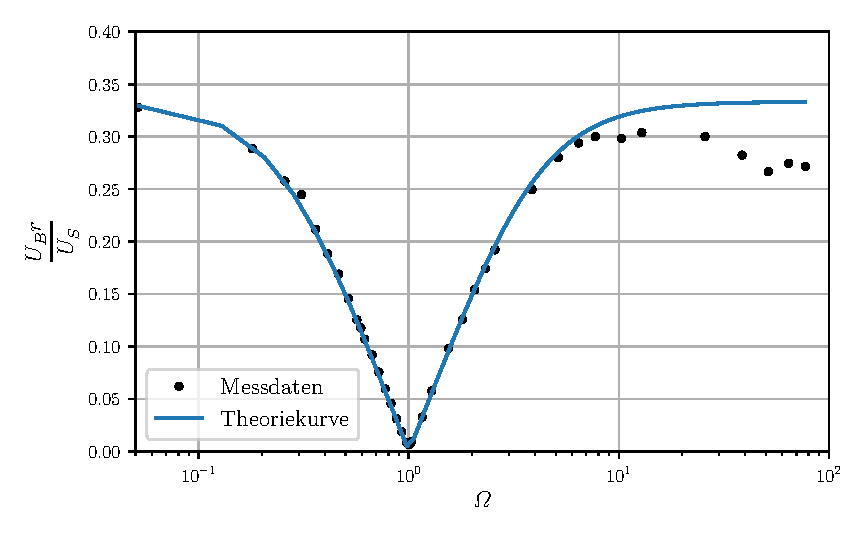
\includegraphics[width = \textwidth]{plot.pdf}
\end{figure}
Die Kurven in der Abbildung zeigen gerade um den Bereich der Frequenz $\nu_0$ große Ähnlichkeit auf.
Für höhere Frequenzen ab ca liegen die Messdaten unterhalb der Theoriekurve.\\
\\
Zur Beurteilung des Generator wollen wir noch den Klirrfaktor bestimmen.
Mit der Annahme, dass die Summe der Oberwellen nur aus der zweiten Oberwelle besteht, ergibt sich der Klirrfaktor zum Quotienten aus $U_1$ und $U_2$.
Es ist zu berücksichtigen, dass die Spannung der zweiten Oberwelle durch die Brückenschaltung geteilt wird.
$U_1$ ist in diesem Fall die Speisespannung $U_{\text{S}}$ bei $\nu_0$.
\begin{align*}
  U_1 &= \SI{20.0}{\volt}\\
  U_2 &= \frac{U_{\text{Br}}}{\sqrt{\frac{(2^2 -1)^2}{9\cdot ((1-2^2)^2 + 9\cdot 2^2)}}}\\
&= \frac{\SI{0.129}{\volt}}{\num{0.1491}} = \SI{0.8654}{\volt}\\
\intertext{Für den Klirrfaktor folgt somit:}
\implies k &= \frac{U_2}{U_1} = \num{4.3268e-2}
\end{align*}